\documentclass{article}
\usepackage{amsmath, amsfonts, amsthm, amssymb}  

\usepackage{secdot}
\usepackage{textcomp}
\usepackage{epsfig}
\usepackage{cprotect}
\usepackage[T1]{fontenc}
\usepackage{epstopdf}
\usepackage{hyperref}
\usepackage{rotating}
\usepackage{graphicx}
\usepackage{caption}
\usepackage{subcaption}
\usepackage{multirow}
\usepackage{setspace}
\usepackage{array}
\usepackage{fancyhdr}
\usepackage{lastpage}
\usepackage[T1]{fontenc}

\usepackage{geometry}
\geometry{letterpaper, left=1in, right=1in, top=1in, bottom=1in}

\pagestyle{fancy}
\fancyhf{}
\rhead{\thepage/\pageref{LastPage}}
\lhead{OSU ECEN 2233 - Logic Design - Fall 2023}
\rfoot{\LaTeX}


% ----- Identifying Information -----------------------------------------------
\newcommand{\myassignment}{Lab 3: Simple Finite State Machines}
\newcommand{\myduedate}{Assigned: Monday 10/16; Due \textbf{Monday 10/30} (midnight)}
\newcommand{\myinstructor}{Instructor: James E. Stine, Jr.}
% -----------------------------------------------------------------------------

\begin{document}
\begin{center}
  {\huge \myassignment} \\
  {\large \myduedate} \\
  \begin{flushright}
  \myinstructor \\
  \end{flushright}
\end{center}

\section{Introduction}

This is a somewhat simpler laboratory but a crucial one.  In this
laboratory we will get our first introduction to sequential logic and
how this works.  Although sequential logic is typically a lot smaller
than combinational designs, it is incredibly valuable in that it
provides most of the intelligence within digital logic.  That is, most
computing devices have several million Boolean gates on them, but
without some mechanism to control the logic, it would never work.

In this laboratory, we are going to use an idea that has been in a
popular textbook that is a little older but we are going to give a new
twist to it~\cite{DBLP:books/daglib/0067158}.  Again, although this
laboratory is relatively simple the importance of this laboratory to
later work will be crucial.  So, it is important to try to
understand the procedure in creating these systems.

The specific class of sequential that we will design in this
laboratory are called Finite State Machines or FSMs.  Although we cover them
in a specific manner in class, they are implemented a tad different
than more traditional methods.  This is mainly due to the complexity
in getting the Hardware Descriptive Language (HDL) to understand what
we want to design.

\section{Background}

Until now, we have only designed combinational circuits. In this lab
we will start with circuits that have distinct states. We once again use
SystemVerilog to specify our design.  As discussed in class, since
FSMs are different in terms of their feedback, they should be
integrated within a Hardware Descriptive Language (HDL) a little
differently to allow the synthesizer to properly design them.

In this lab, you’ll design a finite state machine to control the
taillights of a 1965 Ford
Thunderbird~\cite{DBLP:books/daglib/0067158}. There are three lights
on each side that operate in sequence to indicate the
direction of a turn. Figure~\ref{tbird.png} shows the tail lights and
Figure~\ref{tbird_lights.png} shows
the flashing sequence for (a) left turns and (b) right turns.

Both the car and the flashing sequence occur in various varieties in
other cars as well as other vehicles
(e.g., on bicycle lights).  Nevertheless, this is a great 
exercise to learn how to design a simple Finite State Machine (FSM).

\subsection{Baseline Design}

Let us start with designing the state transition diagram for this
FSM.  Give each state a name and indicate the values of the six outputs
\verb!LC!, \verb!LB!, \verb!LA!, \verb!RA!, \verb!RB!, and
\verb!RC! in each state. Your FSM should take three
inputs: reset, left, and right. The circuit should have the following
properties:
\begin{itemize}
\item On reset, the FSM should enter a state with all lights off.
\item When you press \verb!left!, you should see
  \verb!LA!, then \verb!LA! and \verb!LB!, then \verb!LA!, \verb!LB!,
  and \verb!LC!, 
then finally all lights off again.
\item This pattern should occur even if you release \verb!left! during the
  sequence. If \verb!left! is still down when you return to the lights off
  state, the pattern should repeat.  
\item The operation when \verb!right! is active should be similar
  except with \verb!RA!, \verb!RB! and \verb!RC!.
\item It is up to you to decide what to do if the user makes \verb!left! and
  \verb!right! simultaneously true; make a choice to keep your design easy.
\end{itemize}
\begin{figure} [h!]
  \centering
  \includegraphics[scale=0.4]{Tbird.png}
  \caption{Thunderbird Tail Lights~\cite{DBLP:books/daglib/0067158}}
  \label{tbird.png}
\end{figure}
\begin{figure} [t!]
  \centering
  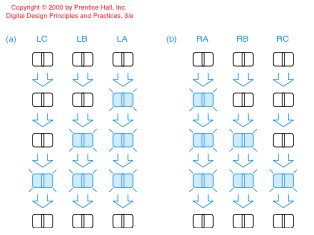
\includegraphics[scale=0.35]{tbird_lights.png}
  \caption{Flashing Sequence (shaded lights are illuminated)~\cite{DBLP:books/daglib/0067158}}
  \label{tbird_lights.png}
\end{figure}

The job of an FSM is to do three things:
\begin{enumerate}
\item Determine the next state from the present state, 
  and the inputs (next state logic).
\item Realize the output function based on the present state and the
  inputs if a Mealy FSM is used (output logic).  
\item Advance from the present state to next state when a clock event
  arrives (state register).
\end{enumerate}
 
As discussed in class, the state-machine diagram is an optional step,
however, the state transition table is an integral and required step
to start.  You should start designing your state-transition table.
Essentially, a state-transition table is a state-machine diagram in
a table form, so that we can use our
knowledge in designing combinatorial circuits to derive the Boolean
equations for next state logic and output logic.

\subsection{FSMs in SystemVerilog}

Again, as discussed in class, synthesis engines must resort to
methodologies that allow them to integrate FSMs into hardware.  There
is an extensive amount of literature on the integration of FSMs, but
it basically boils down to the following items within the HDL.  These
items are basically the same for other HDLs including VHDL and Verilog.

Inside the SystemVerilog file, each FSM has to have the following
distinct and separate items.
\begin{itemize}
\item the state register (where clock moves the next state to the present state)
\item the next state logic (where the next state is determined by the
present state and inputs)
\item the output logic (where the outputs are determined by the present
state and inputs)
works the best.
\end{itemize}

Also discussed in class, the output logic and the next-state logic can
be separate, but I think you will have more luck and less problems if
you combine both of these elements into one item.  We discussed this
in class rather extensively.  Normally, engineers like to have
separate output and next-state logic inside a HDL as it saves space,
but I believe it possibly leads to missing an output.  I will leave
the choice up to you.  The textbook also discusses this rather
extensive in Chapter 4~\cite{ddca-riscv}.

It is also good practice to use a naming style that clearly identifies
the signals that are registered. If you want to know how every
registered signal is connected.  Therefore, you should name your
states accordingly and not something ambiguous like \verb!state1!.

One of the best practices for debugging FSMs is to also make sure you
display your \verb!CURRENT_STATE! and \verb!NEXT_STATE! variables on
the waveform.  This is vital in debugging your FSM and making sure the
output occurs correctly.  You can also output these variables to a
display, such as a $7$-segment display, and many engineers have this
integrated into special debugging configurations for a digital
design.

\subsection{Asynchronous Events and Synchronizing the Clock}

You have described a clock input (\verb!clk!) in your circuit. The question
is where do we get this clock from? You could be tempted to use one of
the push buttons or the switches for this purpose.  I brought this up
in lecture when discussing the time it takes to activate a switch,
such as in Family Feud\textsuperscript{TM} game.  Events that synchronize
events are fairly fast, whereas, outside occurrences are sometimes
slow making putting these events into digital logic sometimes
difficult.

The problem is that compared to the speed of the FPGA the change in a
push button is extremely slow (in fact more than a million times
slower). During the slow transition the FPGA will see many fast
occurring transitions, and would interpret each of them as a clock
edge. This is known as ‘bounce’, and usually specialized circuits (and
sampling techniques) are used to prevent this. In any case, using the
push buttons is not a very safe way of generating the clock.

If you look at your board, you may notice the text
\verb!sysclk_125mhz!. If fact, your board contains a $125$MHz crystal
oscillator circuit. The output of this oscillator is connected to the pin W5
(which is a special clock pin for this FPGA). We will simply tell
he compiler to connect the net “clk” to the pin W5 in the constraints
file (XDC). In this way we will have a clean clock signal.

Now we have a different practical problem: the clock is too fast. The $125$
MHz means that every clock period is $8$ nanoseconds long. The entire
blinking sequence would be then $40$ ns. This is a very short time:
light travels less than $250$ meters during that time. If we want to see
our sequence, we need to find a way to dramatically slow down the
circuit.

This can be achieved by two means. Either we implement a clock divider
circuit that divides the clock by a few million times, or we can
generate an enable signal every few million cycles, and then use this
enable signal to control our next state transition.  We will employ
the former for this laboratory.

In this exercise, we will give you a small \verb!clk_div! circuit that takes
in the same \verb!clk! and \verb!rst! signals, and generates a
\verb!clk_en! edge signal
every $8,388,608$ cycles (or every $2^{23}$ cycles). Considering that
the main clock frequency is $125,000,000$ cycles per second, this means
a \verb!clk_en! signal is generated every $0.06711$ seconds
or $67.11$ ms.  This is a realistic clock to our light controller in action.
The SystemVerilog is shown in Figure~\ref{clk_div.sv}

The idea is pretty simple, we increment a $24$-bit counter (called
\verb!clk_div!) at every clock, and set the \verb!clk_en! to $1$ when
the most-significant bit (MSB) of the counter
s $1$. By increasing the counter size you can
change the division factor as you please.  Use this new \verb!clk_en!
as your clock for your FSM.
Now all we have to do is to choose which buttons on the board we want
to use for the control, and which LEDs we will use as
taillights.
\begin{figure}
\begin{verbatim}
module clk_div (input logic clk, input logic rst, output logic clk_en);

 logic [23:0] clk_count;

 always_ff @(posedge clk)
 //posedge defines a rising edge (transition from 0 to 1)
  begin
   if (rst)
    clk_count <= 24'h0;
   else
    clk_count <= clk_count + 1;
  end
 assign clk_en = clk_count[23];
endmodule
\end{verbatim}
\caption{Clock Divider SystemVerilog File}
\label{clk_div.sv}
\end{figure}


\subsection{Alternate Design}

We also want to make several modifications to this lab to give some
different approaches.  Therefore, you should also incorporate the
following items into your design as a modification of the baseline
laboratory.
\begin{itemize}
  \item If both \verb!left! and \verb!right! are both asserted, you
    should have both lights (e.g., \verb!LA!, \verb!LB!, and
    \verb!LC!) flash on and off.  This would be similar to a hazard
    light in your car.
    \item The Ford Mustang's hazard lights work like the normal
      hazards except they produce them in sequence like our normal
      baseline lab.  That is, you should have them do the following
      when in hazard mode: 1.) \verb!LA! and \verb!RA! 2.) add
      \verb!LB! and \verb!RB! and finally 3.) add \verb!LC! and
      \verb!RC!.  You can see them on the following YouTube video:
      \url{https://youtu.be/5azgaPDvPDk}.
\end{itemize}

You should download the files in this lab from Canvas.  In the
distribution is the normal \verb!top_demo! similar to Laboratory~$1$.
A template FSM SystemVerilog file is given and you can use it to
modify your FSM for this laboratory.  As mentioned in previous labs,
please make sure you adequately simulate your design with a
testbench.  Do not go to implementation without simulating your design
completely on your laptop or desktop at home.

Both the clock divider and template Finite
State Machine SystemVerilog (SV)
file are given to you in your zip files.  There are also separate
\verb!DO! files so you can run both easily.  You will need, as
indicated previously, a complete a state-transition table for your
design.  Although it is tempting to do this without writing it down,
it is highly advisable to write it down.
Then, just update your FSM SV file accordingly.

\subsection{Power, Performance and Area (PPA)}

For this laboratory, we are going to analyze the design with the same
PPA as in previous labs.  That is, you should analyze your design for
Power, Performance
and Area.  Again, as with
any digital design, engineers use PPA to assess the level of
difficulty, challenge, and effort needed for a design.  You should
also generate a schematic of your design by using the tools within
Vivado - this should be an easy click and generate option.  If you
cannot find this, please let us know.

\section{Tasks}

This is a simple lab and just involves implementing the Finite State
Machine for both the baseline and alternate design (i.e., with
hazards).  Of all our labs, this laboratory is probably the easiest,
but FSMs are essential to our project;  therefore, make sure you do
your best to understand how to implement FSMs as well as debug issues
and/or errors that occur.

The main tasks for this laboratory
will be the following elements:
\begin{enumerate}
  \item Design the simple FSM that lights up the LEDs for a Left and
    Right turn.
  \item Implement the alternative design that also has lights for a 
    warning or hazard condition similar to the one found on the YouTube
    video above.
  \item After verifying your design with a testbench in ModelSim,
    implement your design on the DSDB board and use the    
    LEDs for your lights.  You can assign any $3$ LEDs for left and
    $3$ LEDs for right turns.  You should use the switches for initiating a
    Left, Right, or Hazard condition making sure that multiple
    operations do not occur simultaneously.  You should also implement
    a reset for your FSM.
  \item Document your FSM diagram with paper/pencil or a program such
    as graphviz.  It would also be advantageous to have an
    implementation on paper (i.e., using D-flip flops)
    as well as the schematic what is produced from Vivado.
  \item Use the push buttons, switches, and LEDs to help you input
    your plaintext as well as debug operation and prove that your
    design works on your DSDB board.
    \item You should also analyze the PPA impact on your design. 
\end{enumerate}

\subsection{Submission}

You should electronically hand in your HDL (all files that you want
us to see) into Canvas.
You should also take a printout of your waveform 
from your ModelSim simulation and annotate it correctly.  
Only one of your team members should upload
the files and/or lab report. Please contact
James Stine
(james.stine@okstate.edu) 
for more help.  Your
code should be
readable and well-documented. In addition, please turn in additional
test cases or any other added item that you used. 
Please also remember to document everything in your Lab Report using
the information found in the Grading Rubric.


\subsection{Hints/Tips}

One of the challenges in this lab is that the clock for the FSM is so
much slower than the clock for the FPGA.  This will allow you to use a
clock that is faster.  Do not forget to output the
\verb!CURRENT_STATE! and \verb!NEXT_STATE! to your waveform to check
where you are with your state.
It would be highly advisable
to also simulate the FSM with a separate testbench.  Then, create a
top-level module (i.e., digital design) that incorporates the
\verb!clk_en! and the FSM and simulate with a separate testbench than
the \verb!clk_en! and the FSM.  The Graphical User Interface or GUI
is really useful in debugging your FSM. Another great hint
is to also output both
state variables (e.g., as \verb!output logic! instead of \verb!logic! and then send
that output to the board somehow (e.g., $7$-segment display).

As in previous labs, it is highly advisable to do all your simulation
at home before you get to ENDV.  The testbench methodology is so
crucial to the implementation and saves you so much time.  Otherwise,
you are debugging both the implementation and design and just wasting
time.  So, make sure you have your design completely working within a
testbench before you come to ENDV 360.

Also remember there are two types of Finite State Machine (FSM)
designs as discussed in class:
Mealy and Moore.  This lab will implement a Moore-style FSM and you
should define the output per each state.  The book does this a little
differently within SystemVerilog and its far
easier to define the
output in each next-state as recommended, as mentioned in class.

Also, remember you can use the switches, LEDs, push buttons and
$7$-segment displays to help you debug the implementation.  These
debugging elements are very crucial to debugging your design.  Also,
feel free to play with the clock divider to speed or slow things
down.  If you get tricky, you could easily output the time (i.e. in
ms or seconds) that the
clock is working at on the $7$-segment display, which would be a cool
extra-credit option.  

\bibliographystyle{IEEEbib}
\bibliography{lab3}

\end{document}
